\documentclass[12pt,A4,titlepage]{article}
\usepackage[dvipsnames,rgb,dvips,table]{xcolor}
\usepackage{graphicx,caption}
\graphicspath{Figures/}
\usepackage{psfrag}
\usepackage{dcolumn}
\usepackage{bm}
\usepackage{amsmath}
\usepackage{amssymb}
\usepackage[rflt]{floatflt}
\usepackage{latexsym}
%\usepackage{float}
\usepackage{bm}
\usepackage{subcaption}
\usepackage{booktabs}
\usepackage{floatrow}
\floatsetup[table]{font=footnotesize}
\usepackage[hidelinks]{hyperref}


\usepackage{geometry}
 \geometry{
 left=20mm,
 right=20mm,
 top=25mm,
 bottom=20mm,
 }



%\addtolength{\topmargin}{-1.9cm}
%\addtolength{\textheight}{5.5cm}
%\addtolength{\evensidemargin}{-1.2cm}
%\addtolength{\oddsidemargin}{-1.2cm}
%\addtolength{\textwidth}{2cm}


\pagestyle{myheadings}
\markright{{\small Jacopo Credi \hfill (910216-T396) \,}}
\DeclareMathOperator\erf{erf}
\author{Jacopo Credi \\(910216-T396) \\ \vspace*{2cm} }
\title{{\Large \textsc{Chalmers University of Technology}} \\ \bigskip FFR135 - Artificial Neural Networks\\ \bigskip Examples sheet 2 \\ \vspace*{2cm}}

\usepackage{listings}
\usepackage{color} %red, green, blue, yellow, cyan, magenta, black, white
\definecolor{mygreen}{RGB}{28,172,0} % color values Red, Green, Blue
\definecolor{mylilas}{RGB}{170,55,241}
% Settings for writing Matlab code
\lstset{language=Matlab,%
	basicstyle=\small\ttfamily,
    %basicstyle=\color{red},
    breaklines=true,%
    morekeywords={matlab2tikz},
    keywordstyle=\color{blue},%
    morekeywords=[2]{1}, keywordstyle=[2]{\color{black}},
    identifierstyle=\color{black},%
    stringstyle=\color{mylilas},
    commentstyle=\color{mygreen},%
    showstringspaces=false,%without this there will be a symbol in the places where there is a space
    numbers=left,%
    numberstyle={\tiny \color{black}},% size of the numbers
    numbersep=9pt, % this defines how far the numbers are from the text
    %emph=[1]{for,end,break},emphstyle=[1]\color{red}, %some words to emphasise
    frame=single,                   % adds a frame around the code
  	rulecolor=\color{black},
    %emph=[2]{word1,word2}, emphstyle=[2]{style},    
}



\setlength{\parskip}{3pt}


\begin{document}
\parindent=0cm
\maketitle

\subsection*{Problem 1(a)}

\begin{minipage}{0.69\textwidth}
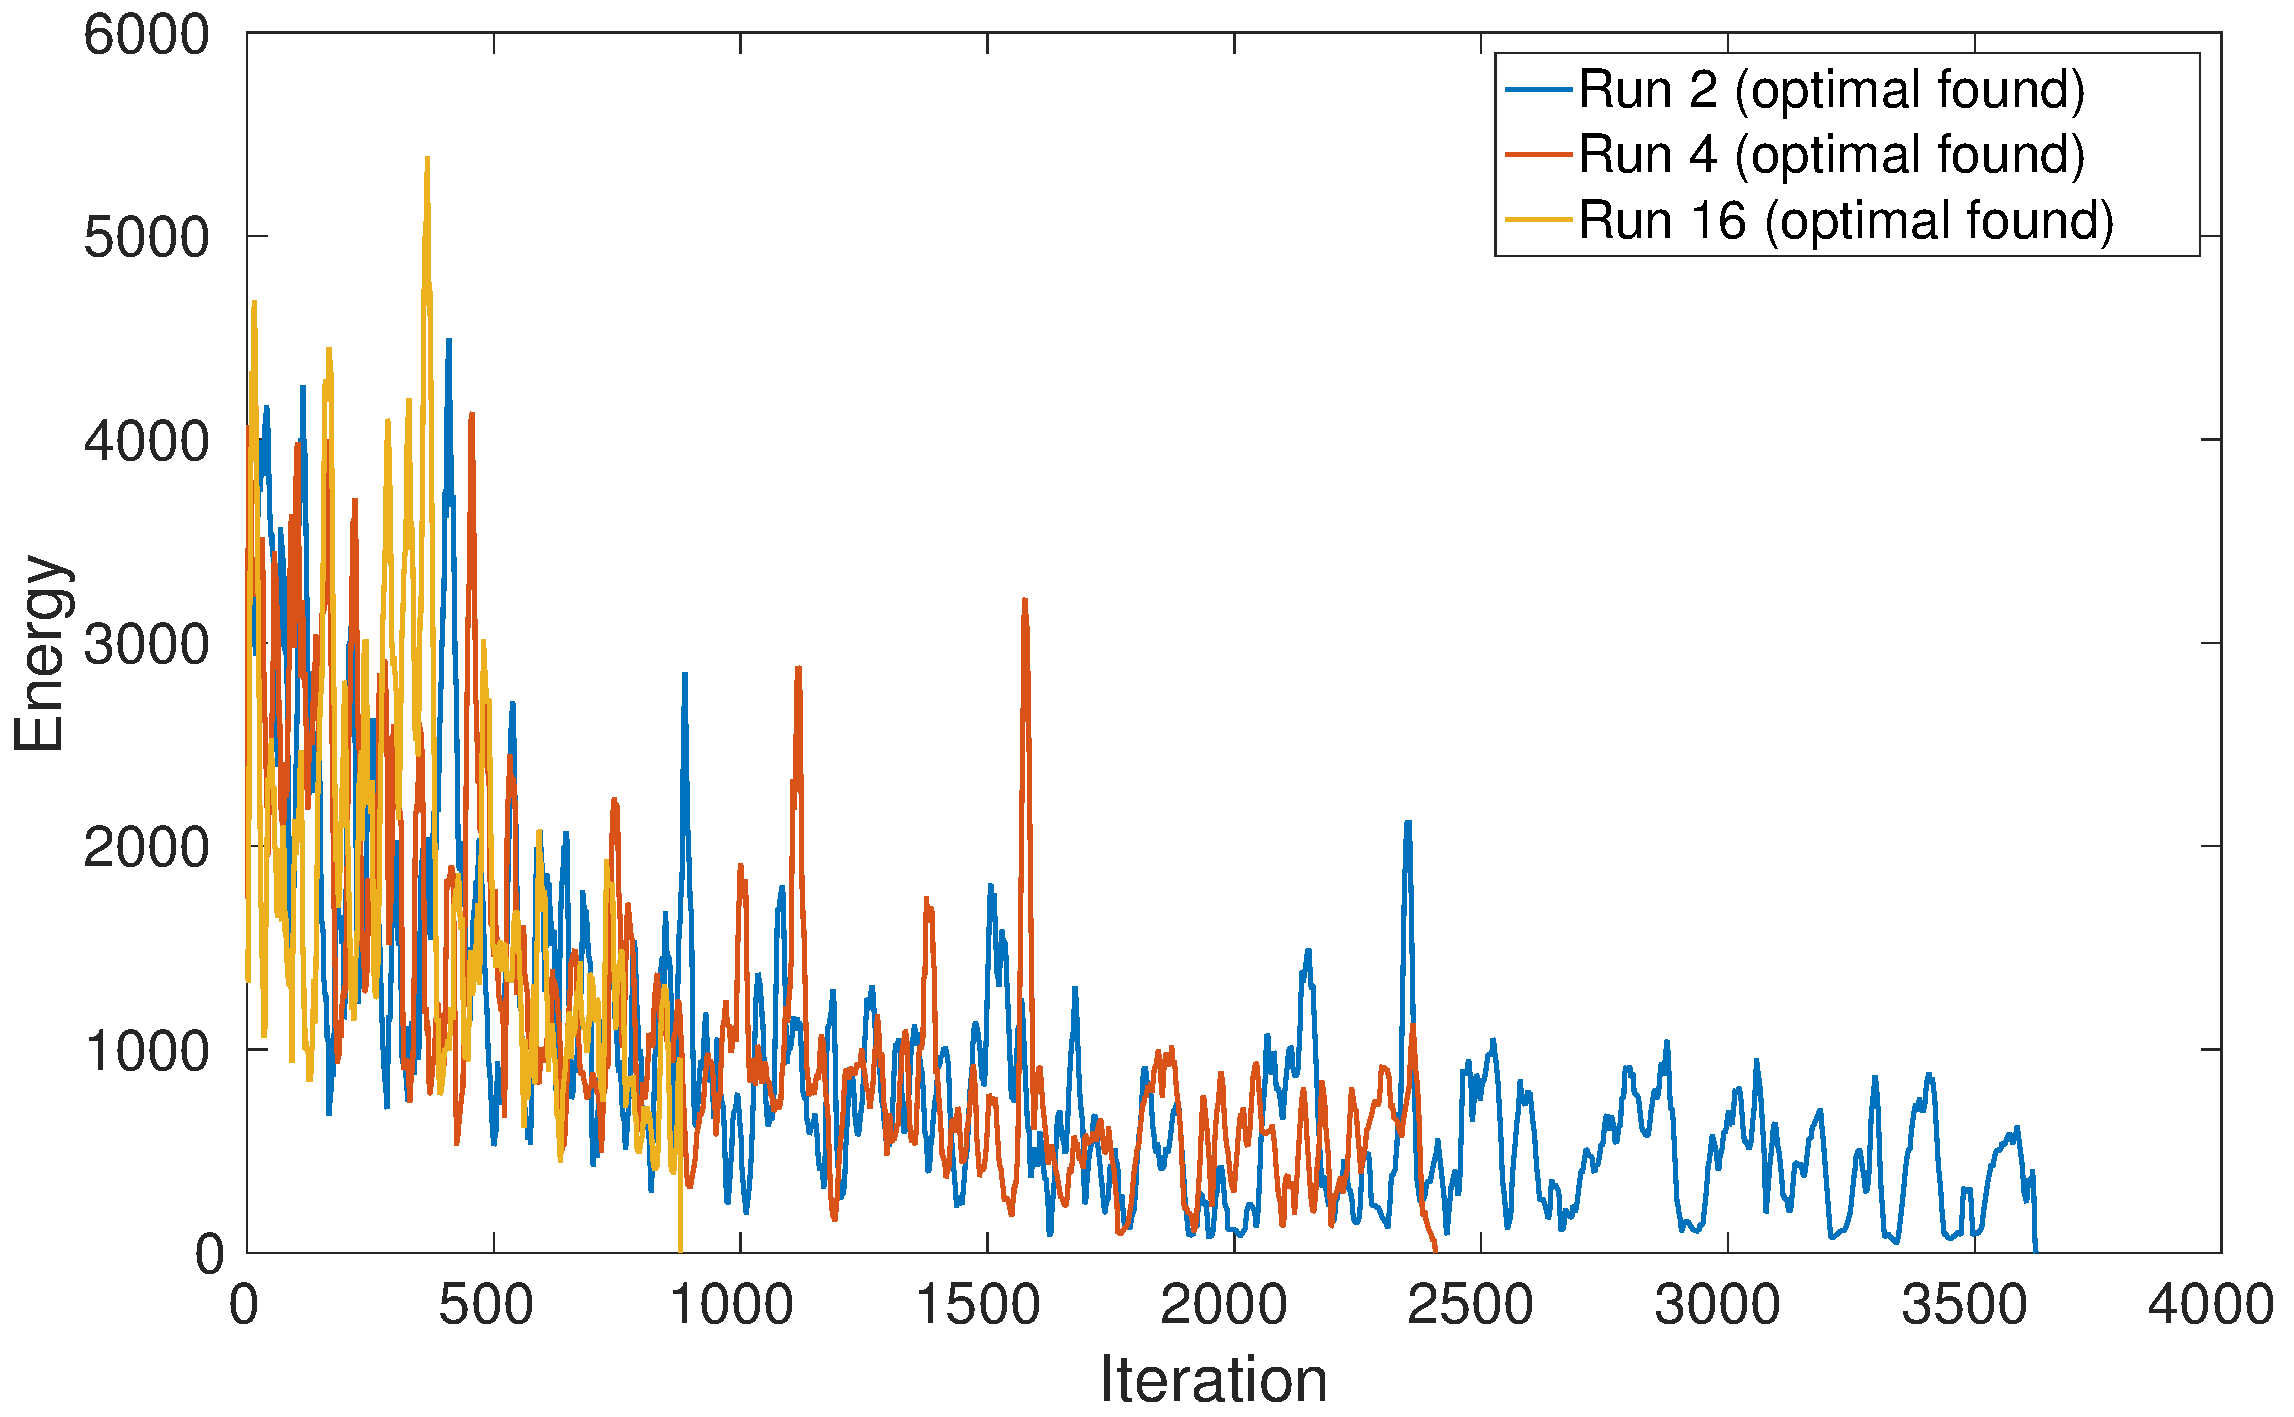
\includegraphics[width=\textwidth]{Figures/1a_energy_1e-6_smooth.pdf}
\captionof{figure}{\footnotesize Evolution of energy over time for 3 runs randomly picked out of 100 runs with noise decrease rate $\alpha = 1\cdot10^{-6}$. Maximum allowed iterations $t_{\textup{max}}=5\cdot10^4$. A moving average with a span of $20$ points is displayed for clarity.}
\label{1aFig}
\end{minipage}\hfill\begin{minipage}{0.28\textwidth}
\vfill
\resizebox{\textwidth}{!}{
\begin{tabular}{ccc}
\toprule
$\alpha$ & Optimal & $\left<t_{\textup{conv}}\right>$ \\
\midrule
%$1\cdot10^{-3}$ & $29\%$ & $265$ \\
$3\cdot10^{-4}$ & $32\%$ & $346$ \\
$1\cdot10^{-4}$ & $45\%$ & $415$ \\
$3\cdot10^{-5}$ & $46\%$ & $552$ \\
$1\cdot10^{-5}$ & $71\%$ & $985$ \\
$3\cdot10^{-6}$ & $90\%$ & $1914$ \\
$\bm{1\cdot10^{-6}}$ & $\bm{97}$\textbf{\%} & $\bm{2810}$\\
$3\cdot10^{-7}$ & $93\%$ & $3818$ \\
$1\cdot10^{-7}$ & $76\%$ & $3983$ \\
$3\cdot10^{-8}$ & $71\%$ & $4002$ \\
$1\cdot10^{-8}$ & $67\%$ & $4129$ \\
\bottomrule
\end{tabular}}
\captionof{table}{\footnotesize Fraction of optimal solutions and average convergence time as a function of noise decrease rate $\alpha$. Values were obtained by performing $100$ runs for each value of $\alpha$. Maximum allowed iterations $t_{\textup{max}}=5\cdot10^4$.}
\vfill
\label{1aTable}
\end{minipage}

%\subsubsection*{Discussion}

\bigskip
A \textsc{matlab} implementation of the simulated-annealing algorithm was applied to \verb!data_1!, with parameter $\beta$ increasing linearly over time $\beta = \alpha \cdot t$ and candidate configuration being sampled in the neighbourhood of current configuration, as defined in Goldstein and Waterman (1987). 

The energy evolution over time, plotted in Fig.~\ref{1aFig} for three randomly chosen runs, reflects the expected behaviour for the SA algorithm. In the beginning, when the noise level is high, energy exhibits large fluctuations, which are then damped over time as the system is ``cooled down''. The average value of the energy decreases over time, since configurations $(\sigma,\mu)$ which causes the energy to decrease are more likely to be accepted.

The percentage of runs in which an optimal solution was found (i.e. the energy reaches zero) was observed to depend critically on $\alpha$, and the same applies for the average number of iterations needed to reach zero energy, based on the runs in which an optimal solution was found (see Table~\ref{1aTable}). 

The observed trends can be explained as follows: if $\alpha$ is too large, the system is cooled down too quickly and a large fraction of Markov Chains get stuck in a local minimum, but those chains which do converge to zero do so very quickly (e.g. $\left<t_{\textup{conv}}\right> = 552 \ $ when $\ \alpha = 3\cdot10^{-5}$). On the other hand, if $\alpha$ is too low, the simulated annealing method has little advantage over a purely random search, and as $\alpha$ is decreased $\left<t_{\textup{conv}}\right>$ increases, and a larger and larger fraction of MC do not converge within the specified maximum number of iterations $t_{\textup{max}} = 5\cdot10^4$, even though they would probably converge if this value was larger.

With this value of $t_{\textup{max}}$, a noise decrease rate $\alpha = 1\cdot10^{-6} \ $ (in bold in Table~\ref{1aTable}) yields the largest percentage of optimal solutions and the lower runtime of the implemented program (as almost all chains converge to $H(S^{(k)}) = 0$ in a few thousands steps, well before $t_{\textup{max}}$ is reached).

\vspace*{-0.2cm}
\subsubsection*{Reference code}
See \textsc{matlab} script \verb!Main.m! and custom functions called in the script itself.

\clearpage


\subsection*{Problem 1(b)}

\begin{table}[H]
\resizebox{\textwidth}{!}{
\begin{tabular}{ccccc}
\toprule
Solution ID & Permutation $\sigma$ & Permutation $\mu$ & Resulting permutation of \textbf{c} & Energy \\
\midrule
$(1)$ & $( a_1 \ a_6 \ a_4 \ a_2 \ a_3 \ a_5)$ & $(b_1 \ b_2 \ b_6 \ b_3 \ b_5 \ b_4)$ & $(c_1 \ c_{11} \ c_3 \ c_7 \ c_2 \ c_6 \ c_9 \ c_4 \ c_8 \ c_5 \ c_{10})$ & 0\\
$(2)$ & $( a_1 \ a_6 \ a_4 \ a_2 \ a_3 \ a_5)$ & $(b_1 \ b_2 \ b_5 \ b_3 \ b_6 \ b_4)$ & $(c_1 \ c_{11} \ c_3 \ c_7 \ c_2 \ c_6 \ c_8 \ c_4 \ c_9 \ c_5 \ c_{10})$  & 0\\
$(3)$ & $( a_5 \ a_3 \ a_2 \ a_4 \ a_6 \ a_1)$ & $(b_4 \ b_5 \ b_3 \ b_6 \ b_2 \ b_1)$ & $(c_{10} \ c_5 \ c_8 \ c_4 \ c_9 \ c_6 \ c_2 \ c_7 \ c_3 \ c_{11} \ c_1)$  & 0\\
\bottomrule
\end{tabular}}
\caption{\footnotesize Three optimal solutions found for \texttt{data\_1}. The solution ID has no particular meaning and was just introduced for convenience. They were not chosen randomly, though, but in order to illustrate a point.}
\label{1bTable}
\end{table}

\vspace*{-0.2cm}
In general, the double-digest problem (DDP) has multiple optimal solutions. Three of the optimal solutions found by the implemented SA algorithm are shown in Table~\ref{1bTable}, but many more were found.

It was observed that solutions (2) and (3) in Table~\ref{1bTable}, in particular, can be reconstructed from solution (1). Permutation $\sigma^{(2)}$, in fact, is exactly the same as permutation $\sigma^{(1)}$, whereas permutation $\mu^{(2)}$ can be obtained from permutation $\mu^{(1)}$ by swapping elements $b_5$ and $b_6$. Why does such a swap lead to a different optimal solution? Because in solution (1) the sub-portion $(b_6 \ b_3 \ b_5)$ is completely ``contained'' in element $a_3$ (as illustrated in yellow in Fig.~\ref{1bFig}), therefore swapping any couple of these elements results in a zero-energy solution.

\begin{figure}[H]
\centering
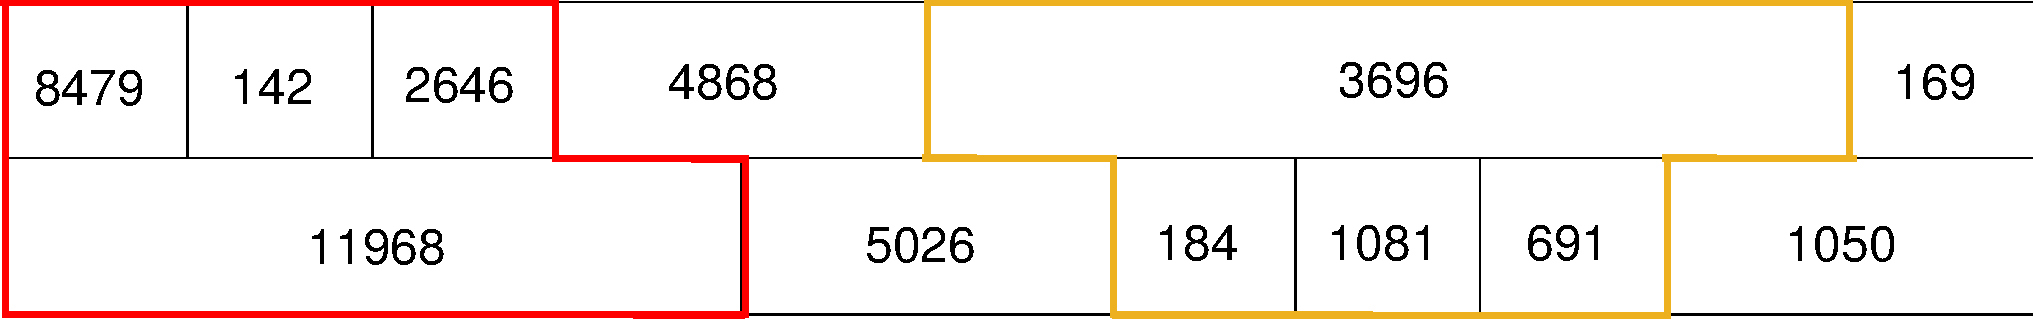
\includegraphics[width=0.7\textwidth]{Figures/blocks.pdf}
\caption{\footnotesize Graphical representation of solution (1) in Table \ref{1bTable}. The drawing is not to scale.}
\label{1bFig}
\end{figure}

\vspace*{-0.2cm}
We can indeed calculate the number of optimal solutions that can be constructed starting from solution (1) by \emph{swapping} fragments in $\sigma^{(1)}$ contained in some $b_i \in$ $\mu^{(1)}$ and viceversa. As made clear by Fig.~\ref{1bFig}, three fragments in $\sigma^{(1)}$, namely $a_1 = 8479$, $a_6 = 142$ and $a_4 = 2646$, are completely contained in $b_1 = 11968$ (see red box), and three fragments in $\mu^{(1)}$, namely $b_6 = 184$, $b_3 = 1081$ and $b_5 = 691$, are completely contained in $a_3 = 3696$ (see yellow box). Any couple of fragments within these triples can be swapped and the result will also be an optimal solution. The number of such allowed swaps is $3! \ 3! = 36$, thus there are at least $36$ optimal solutions.

Moreover, any sequence obtained by \emph{reflecting} an optimal solution is also an optimal solution. For instance, solution (3) in Table~\ref{1bTable} is nothing but the reflection of solution (1). Therefore, we can conclude that the total number of optimal solutions for \texttt{data\_1} is 
\vspace*{-0.1cm}\[
N_{\textup{opt}} = 2 \cdot 3! \cdot 3! = 72 \ .
\]

\vspace*{-0.1cm}
Since the configuration space for this problem is relatively small ($6! \ 6! = 518400$ configurations), a complete search was performed, verifying that indeed the number of optimal solution is 72.

\vspace*{-0.2cm}
\subsubsection*{Reference code}
See \textsc{matlab} script \verb!Main.m! and custom functions called in the script itself, in particular\\ \verb!CountSolutions.m! and \texttt{CompleteSearch.m}.

\clearpage



\subsection*{Problem 1(c)}

A double-digest problem is completely specified by giving sequences
\begin{align*}
\bm{a} &= \lbrace a_1, \ldots, a_n \rbrace \qquad \text{with} \quad a_1 \geq a_2 \geq \ldots a_n \ , \\
\bm{b} &= \lbrace b_1, \ldots, b_m \rbrace \qquad \text{with} \quad b_1 \geq b_2 \geq \ldots b_m \ , \\
\bm{c} &= \lbrace c_1, \ldots, c_l \rbrace \qquad \ \text{with} \quad c_1 \geq c_2 \geq \ldots c_l \ . \\
\end{align*}
There are $n!/q!$ possible permutations of sequence $\bm{a}$, where $q$ is the number of repeated elements in $\bm{a}$, and $m!/r!$ possible permutations of sequence $\bm{b}$, where $r$ is the number of repeated elements in $\bm{b}$. The size of the configuration space for such a problem is therefore given by
\[
N = \dfrac{n! \ m!}{q! \ r!} \ .
\]
The probability of sampling the correct solution it out of $N$ possible configuration if picking randomly is
\begin{equation}
p = \dfrac{1}{N} = \dfrac{q! \ r!}{n! \ m!} \ ,
\end{equation}
thus the probability of sampling the correct configuration after $t$ unsuccessful samples is
\begin{equation}
P(\text{``success after $t$ trials''}) = (1-p)^t \ p = p \ e^{t \ \log(1-p)} \simeq p \ e^{-pt} \ ,
\label{psuccess}
\end{equation}
where the last approximation comes from the Taylor expansion 
\[
\log(1-x) = -x + o(x) \quad \text{for} \quad x \rightarrow 0 \ .
\]
In our case (\texttt{data\_1}) we have $n = m = 6$ and $q = r = 0$, therefore $p = 1/518400 \simeq 1.929\cdot10^{-6}$ and the approximation can be considered sufficiently good. 

Equation~(\ref{psuccess}) allows us to approximate the average number of iterations needed to find the correct sequence under a random search as the expected value of a random variable $T_{\textup{correct}} \sim \text{Exp}(p)$, i.e. exponentially distributed with parameter $p$:
\begin{equation}
\mathbb{E}(T_{\textup{correct}}) \simeq\footnotemark \int_0^\infty t \ p \ e^{-p\ t} \ dt = \Bigl[ -t \ e^{-p\ t} \Bigr]_0^{\infty} - \int_0^\infty e^{-p\ t} \ dt = \dfrac{1}{p} = \dfrac{n! \ m!}{q! \ r!} \ .
\end{equation}
\footnotetext{Here we are neglecting a correction factor of $e^p \sim 1.000001929$}

The expected number of iterations needed for a random search to find the correct solution is therefore equal to the size of the configuration space, i.e. for \texttt{data\_1} we have
\[
\mathbb{E}(T_{\textup{correct}}) \simeq 518400 \ .
\]

In comparison, the average number of iterations needed by the SA algorithm to find \emph{an} optimal solution is 2 to 3 orders of magnitude lower (see Table~\ref{1aTable}). And even if the \emph{optimal} solution found by the SA method might not be the \emph{correct} one, once an optimal solution has been found, the set of other optimal solutions can be reconstructed by applying appropriate transformations.
\clearpage



\subsection*{Problem 2(a)}

\begin{table}[H]
\resizebox{\textwidth}{!}{
\begin{tabular}{lrlc}
\toprule
 & & Optimal configurations (zero energy) found for \texttt{data\_2} &\\
\midrule
& $\sigma^{(1)} =$ &$( a_8 \ a_6 \ a_4 \ a_{10} \ a_9 \ a_1 \ a_2 \ a_5  \ a_3 \ a_7)$ \\
(1) & $\mu^{(1)} =$ &$(b_8 \ b_6 \ b_7 \ b_2 \ b_1 \ b_4 \ b_{11} \ b_3 \ b_9 \ b_5 \ b_{10} )$\\
& Resulting \textbf{c} sequence $=$ &$(c_{10} \ c_{16} \ c_8 \ c_{18} \ c_{11} \ c_6 \ c_{15} \ c_{14} \ c_4 \ c_2 \ c_5 \ c_3 \ c_7 \ c_{20} \ c_{12} \ c_1 \ c_{17} \ c_{13} \ c_9 \ c_{19})$\\
 & Iterations for convergence $=$ & $481441$ \\
\midrule
& $\sigma^{(2)} =$ &$( a_7 \ a_3 \ a_5 \ a_2 \ a_1 \ a_{10} \ a_9 \ a_4  \ a_6 \ a_8)$ \\
(2) & $\mu^{(2)} =$ &$(b_{10} \ b_5 \ b_9 \ b_3 \ b_{11} \ b_4 \ b_1 \ b_2 \ b_7 \ b_6 \ b_8 )$\\
& Resulting \textbf{c} sequence $=$ &$(c_{19} \ c_9 \ c_{13} \ c_{17} \ c_1 \ c_{12} \ c_{20} \ c_7 \ c_3 \ c_5 \ c_2 \ c_4 \ c_{15} \ c_{14} \ c_6 \ c_{11} \ c_{18} \ c_{8} \ c_{16} \ c_{10})$\\
 & Iterations for convergence $=$ & $563669$ \\
\bottomrule
\end{tabular}}
\caption{Optimal solutions found for \texttt{data\_2} by the implemented SA algorithm with $\alpha = 10^{-7}$.}
\label{2aTable}
\end{table}

The simulated-annealing algorithm was successfully applied to solve the DDP specified in \texttt{data\_2}, finding two optimal solutions (zero energy) displayed in Table~\ref{2aTable}.

In order to obtain these solutions, the algorithm was tested for several values of $\alpha$, performing up to $10^6$ iterations per run. The optimal solutions displayed above were then found by setting $\alpha = 10^{-7}$ and completing $50$ runs, each with a maximum allowed number of iterations $t_{\textup{max}}=7.5\cdot10^5$. Under these conditions, the percentage of successful runs was $4\%$ and the average number of iterations needed for convergence to optimum was $\left<t_{\textup{conv}}\right> = 522555$.

As expected, the optimal solution is not unique. Again, we can notice that solution (2) can be constructed from solution (1), by reflecting it and then swapping fragments $a_{10}$ and $a_9$. Two more optimal solutions can therefore be obtained by transforming solution (1): one by reflecting it without swapping fragments $a_{10}$ and $a_9$, and another one by swapping fragments $a_{10}$ and $a_9$ without reflection. This leads us to claim that there are 4 optimal solutions for this double-digest problem.

In comparison with \texttt{data\_1}, this DDP seems to have fewer solutions, even though the number of fragments is larger. This is possible, albeit counterintuitive at first, because a larger number of fragments in sequence \textbf{c} means a larger number of constraints to satisfy in order for a solution to be optimal.

The difficulties in finding an optimal solution were expected, as the configuration space for this problem is much larger than the one in \texttt{data\_1} (see \textbf{Problem 2b}).

\vfill
\subsubsection*{Reference code}
See \textsc{matlab} script \verb!Main.m! and custom functions called in the script itself.

\clearpage
 
\subsection*{Problem 2(b)} 
 
In order to estimate the expected number of iterations needed to find the \emph{correct} solution under a purely random search for DDP in \texttt{data\_2}, we can use the approximation derived in part \textbf{1c} (Equation (3)). Since here $n \equiv \mid \bm{a} \mid = 10$, $\ m \equiv \mid \bm{b} \mid = 11$, and $\ q = r = 0$, we have
\[
\mathbb{E}(T_{\textup{correct}}) \ \simeq \ \dfrac{n! \ m!}{q! \ r!} \ = \dfrac{10! \ 11!}{1} \ = 144850083840000 \ \simeq \ 1.45 \cdot 10^{14} \ .
\]

Clearly, the expected number of iterations needed to find the \emph{correct} solution scales extremely quickly with the number of elements in sequences \textbf{a} and \textbf{b}. While in \textbf{Problem 1} it was even possible to perform a \emph{complete} search over the entire configuration space, now this is unthinkable (on my laptop, at least).

The simulated-annealing algorithm, instead, did find a solution (even if it might not be the \emph{correct} one) in about $5\cdot10^5$ iterations. This corresponds to a performance increase of 9 orders of magnitude, making the SA method a much better choice when dealing with this kind of combinatorial problems, even more so as the problem size increases.
 
\clearpage

\appendix








\section*{Appendix: MATLAB code}

\subsection*{\texttt{Main.m}}

\begin{lstlisting}
%MAIN
clear

% ================================================================= %
% Parameters
% ================================================================= %

% Use either data from data_1.rtf or data_2.rtf
a=[9979, 9348, 8022, 4020, 2693, 1892, 1714, 1371, 510, 451];
b=[9492, 8453, 7749, 7365, 2292, 2180, 1023, 959, 278, 124, 85];
c=[7042, 5608, 5464, 4371, 3884, 3121, 1901, 1768, 1590, 959, 899, 707, 702, 510, 451, 412, 278, 124, 124, 85];

nRuns = 50;
maxTime = 750000; % use 50000 for data1, 750000 for data2
alpha = 1e-7; % 1e-6 for data1, 1e-7 for data2

% ================================================================= %

% Initialize output cell array
solutions = repmat(struct('a',a,'b',b,'c',c,'energy',1:maxTime,...
    'isOptimal',false,'runTime',nan), nRuns, 1 );

%% Main (parallel) loop
p =  TimedProgressBar( nRuns, 30, ...
    'Computing... Estimated time left: ', '   Completed: ', 'Completed in ' );
parfor run = 1:nRuns
    solutions(run) = DoubleDigestSimulatedAnnealing( a, b, c, maxTime, alpha);
    p.progress;
end
p.stop;
[ differentSolutions, nSolutions] = CountSolutions( solutions );

% Print some output to console
fprintf('\nFraction of optimal solutions: %f\n', ...
    mean(cell2mat(extractfield(solutions,'isOptimal'))));
fprintf('Average number of iterates for convergence to optimal: %i\n', ...
    int32(nanmean(extractfield(solutions,'runTime'))));
fprintf('Number of different optimal solutions found: %i\n', nSolutions);


%[f1, f2, f3, which] = PlotEnergy(solutions);

delete('timedProgressbar_Transient(deleteThis)_*.txt');
\end{lstlisting}

\subsection*{\texttt{DoubleDigestSimulatedAnnealing.m}}

\begin{lstlisting}
function solution = DoubleDigestSimulatedAnnealing(seqA, seqB, trueC, maxTime, alpha)
%DOUBLEDIGESTSIMULATEDANNEALING
%  solution = DoubleDigestSimulatedAnnealing(seqA, seqB, trueC, maxTime, alpha)
%
%  This function performs a simulated annealing search of an optimal
%  sequence solving the double digest problem. 
%
%  INPUTS: 
%   - sequence a (digested by A)
%   - sequence b (digested by B)
%   - sequence c (digested by both A and B)
%   - max allowed number of iterations
%   - increase rate for beta (it's also starting value for beta at t=1)
%
%  OUTPUT variable is a structure with the following fields:
%   - solution.a : best a-sequence found
%   - solution.b : best b-sequence found
%   - solution.c : best c-sequence found
%   - solution.energy : evolution of energy over time
%   - solution.isOptimal : logical value, true if the found sequence is optimal
%   - solution.runTime : number of iterations needed to find optimal (this value is NaN if optimal solution was not found)

%% Preliminary operations and initializations
nA = numel(seqA);
nB = numel(seqB);
energy = zeros(1,maxTime);
beta = alpha;
time = 1;
isOptimal = false;
runTime = nan;

% Initial guesses (random permutations)
guessA = seqA(randperm(nA));
guessB = seqB(randperm(nB));

% Initialize random logical 1d array (which to update between sigma and mu)
whichToUpdate = rand(maxTime+1,1) > 0.5;

% Corresponding c and initial energy
cTilde = DigestAB(guessA, guessB);
energy(time) = ComputeEnergy( trueC, cTilde);

%% Main loop
while time < maxTime
    
    time = time + 1;
    
    % Make new guesses for sequences a and b and corresponding sequence c
    if whichToUpdate(time) % update sigma
        newGuessA = SampleNeighbourPermutation(guessA);
        newGuessB = guessB;
    else % update mu        
        newGuessA = guessA;     
        newGuessB = SampleNeighbourPermutation(guessB);
    end
    cTilde = DigestAB(newGuessA, newGuessB);

    % Compute newEnergy and decide whether to accept new permutations
    newEnergy = ComputeEnergy( trueC, cTilde);
    
    if AcceptUpdate( beta, newEnergy, energy(time-1));
        guessA = newGuessA;
        guessB = newGuessB;
        energy(time) = newEnergy;
    else
        energy(time) = energy(time-1);
    end
    
    % Check whether an optimal configuration was found
    if newEnergy == 0
        isOptimal = true;
        runTime = time;
        energy(time+1:end) = [];
        break
    end
    
    % Update beta
    beta = alpha*time;
end

solution.a = guessA;
solution.b = guessB;
solution.c = cTilde;
solution.energy = energy;
solution.isOptimal = isOptimal;
solution.runTime = runTime;

end
\end{lstlisting}

\subsection*{SampleNeighbourPermutation.m}

\begin{lstlisting}
function newPermutation = SampleNeighbourPermutation( permutation )
%SAMPLENEIGHBOURPERMUTATION
%  newPermutation = SampleNeighbourPermutation( permutation ) returns an
%  output vector containing the same elements as the input vector, in the
%  same order except for 2 elements, which are swapped.

newPermutation = permutation;

toSwap = randperm(numel(permutation),2);

newPermutation(toSwap) = permutation(fliplr(toSwap));

end
\end{lstlisting}

\subsection*{DigestAB.m}

\begin{lstlisting}
function [ sortedC ] = DigestAB( sequenceA, sequenceB)
%DIGESTAB
%   [ sortedC ] = DigestAB( sequenceA, sequenceB, L ) returns the sorted
%   sequence c that would result from double digestion if sequenceA and
%   sequenceB were the correct fragment sequences. L is the sum of the
%   fragments' lengthts.

% Compute vectors of cumulative sums
cumulatedA = cumsum(sequenceA);
cumulatedB = cumsum(sequenceB);

% Concatenate cumsums and sort the resulting vector
sortedCumulatedC = union(cumulatedA, cumulatedB);

% Compute difference between adjacent elements
sequenceC = diff(sortedCumulatedC);

% Append first element of cumulative sum
sequenceC = [sortedCumulatedC(1) sequenceC];

% Sort resulting vector in descending order
sortedC = sort(sequenceC,'descend');

end


\end{lstlisting}


\subsection*{ComputeEnergy.m}

\begin{lstlisting}
function [ H ] = ComputeEnergy( c, cTilde )
%COMPUTEENERGY
%  H = ComputeEnergy( c, cTilde ) returns the energy function H(S^(k))
%  evaluated at the sequences c, cTilde

maxIndex = min(numel(c),numel(cTilde));
c = c(1:maxIndex);
cTilde = cTilde(1:maxIndex);

H = sum(((c-cTilde).^2)./c);

end
\end{lstlisting}



\subsection*{AcceptUpdate.m}

\begin{lstlisting}
function [ acceptUpdate ] = AcceptUpdate( beta, newH, oldH )
%ACCEPTUPDATE
%  acceptUpdate = AcceptUpdate( beta, newH, oldH ) returns the logical 
%  value 1 (true) if the proposed update with energy newH is accepted, 0
%  (false) otherwise.

deltaH = newH - oldH;

% Compute acceptance probability
if deltaH > 0
    acceptanceProbability = exp(-beta*deltaH);
else
    acceptanceProbability = 1;
end

% Check whether the update is accepted or not
if rand < acceptanceProbability
    acceptUpdate = true;
else
    acceptUpdate = false;
end

end
\end{lstlisting}



\subsection*{CountSolutions}

\begin{lstlisting}
function [structDiffSolutions, nSolutions] = CountSolutions(outputData)
%COUNTSOLUTIONS

nRuns = length(outputData);
nA = numel(outputData(1).a);
nB = numel(outputData(1).b);

aSequences = extractfield(outputData, 'a');
aSequences = reshape(aSequences',[nA nRuns])';

bSequences = extractfield(outputData, 'b');
bSequences = reshape(bSequences',[nB nRuns])';

% Remove non-optimal solutions
isOptimal = cell2mat(extractfield(outputData,'isOptimal'))';
aSequences(~isOptimal,:) = [];
bSequences(~isOptimal,:) = [];

solutionsMatrix = [aSequences, bSequences];

differentSolutions = unique(solutionsMatrix,'rows');

nSolutions = size(differentSolutions, 1);

structDiffSolutions = repmat(struct('a', [] ,'b', []), nSolutions, 1);
    
for k = 1:nSolutions
    structDiffSolutions(k).a = differentSolutions(k,1:nA);
    structDiffSolutions(k).b = differentSolutions(k,nA+1:end);
end

end
\end{lstlisting}


\subsection*{PlotEnergy.m}

\begin{lstlisting}
function [f1, f2, f3, which] = PlotEnergy(solutions)
%PLOTENERGY

% randomly pick 3 chains
which = randi(length(solutions),[1 2]);
which = sort(which);

% if moving average
span = 5000;

smooth1 = smooth(solutions(which(1)).energy, span);
smooth2 = smooth(solutions(which(2)).energy, span);
smooth3 = smooth(solutions(which(3)).energy, span);

figure('units','normalized','outerposition',[0 0 1 1]);
f1 = plot(smooth1, 'LineWidth', 2);
hold on
f2 = plot(smooth2, 'LineWidth', 2);
f3 = plot(smooth3, 'LineWidth', 2);
hold off

% if all data points
% figure('units','normalized','outerposition',[0 0 1 1]);
% f1 = plot(solutions(which(1)).energy, 'LineWidth', 1.5);
% hold on
% f2 = plot(solutions(which(2)).energy, 'LineWidth', 1.5);
% f3 = plot(solutions(which(3)).energy, 'LineWidth', 1.5);
% hold off

set(gcf,'color','w');
set(gca,'fontsize', 28);

xlabel('Iteration');
ylabel('Energy');
pbaspect([1.618 1 1]);

for k = 1:3
    if solutions(which(k)).isOptimal
        converged{k} = ' (optimal found)';
    else
        converged{k} = ' (optimal not found)';
    end
end

str1 = ['Run ',num2str(which(1)), converged{1}];
str2 = ['Run ',num2str(which(2)), converged{2}];
str3 = ['Run ',num2str(which(3)), converged{3}];

legend([f1, f2, f3], str1, str2, str3);

end
\end{lstlisting}


\subsection*{CompleteSearch.m}

\begin{lstlisting}
function [nOptimalSolutions] = CompleteSearch( a, b, c )
%COMPLETESEARCH
%   Search all configuration space for optimal solutions of the DDP
%   specified by sequences a, b, c in input.
%   Returns number of optimal solutions.

% Save memory
if max([a, b]) < 65535
    a = uint16(a);
    b = uint16(b);
end

nOptimalSolutions = 0;

permA = perms(a);
permB = perms(b);

nA = size(permA,1);
nB = size(permB,1);

h = waitbar(0, 'Please wait...');
for aa = 1:nA
    
    tic
    currentA = permA(aa,:);
    
    parfor bb = 1:nB
        if isequal(c,DigestAB(currentA,permB(bb,:)));
            nOptimalSolutions = nOptimalSolutions + 1;
        end
    end
    waitbar(aa/nA, h);
    toc
end
close(h);

toc

end
\end{lstlisting}

\subsection*{\texttt{TimedProgressBar.m}}

This is a nice function to print a waitbar on console when using parallelised for-loops. I found it on MatlabCentral/FileExchange. Credits:  Antonio Jose Cacho.

URL: \url{https://www.mathworks.com/matlabcentral/fileexchange/46763-timedprogressbar})

(Code is not reported here, see the above link.)

\end{document}
